\documentclass[usenatbib,usegraphicx,letterpaper]{mn2e}
\usepackage[totalwidth=480pt,totalheight=680pt]{geometry}

\usepackage{amssymb}
\usepackage{epsfig}
\usepackage{amsmath}
\usepackage{color}
\usepackage[dvipsnames]{xcolor}
%\usepackage{hyperref}
\usepackage{yfonts}

\usepackage{epsfig}  \usepackage{graphicx}   \usepackage{rotating}

%------- New commands

\newcommand{\lsim}{\lower0.6ex\vbox{\hbox{$ \buildrel{\textstyle <}\over{\sim}\ $}}}
\newcommand{\gsim}{\lower0.6ex\vbox{\hbox{$ \buildrel{\textstyle >}\over{\sim}\ $}}}
\newcommand{\beq}{\begin{equation}}
\newcommand{\eeq}{\end{equation}}

%------ Journals

\newcommand{\mnras}{Mon. Not. R. Astron. Soc.}
\newcommand{\apjl}{Astrophys. J. Lett.}
\newcommand{\aj}{Astron. J.}
\newcommand{\aap}{Astron. Astrophys.}
\newcommand{\araa}{Ann. Rev. Astron. Astroph.}
\newcommand{\apjs}{Astrophys. J. Suppl. Ser.}
\newcommand{\physrep}{Phys. Rep.}
\newcommand{\jcap}{JCAP}
\newcommand{\prd}{Phys. Rev. D}
\newcommand{\apj}{ApJ}

\newcommand{\wprp}{w_{\mathrm{p}}}
\newcommand{\rp}{r_{\mathrm{p}}}

\bibliographystyle{mn2e}

%Title of paper---------------------------------------------------------


\title[Clustering Constraints on Assembly Bias]
{
Constraints on Assembly Bias from Galaxy Clustering
}

% Authors ------------------------------------------------------


\author[Zentner et al.]
{Andrew R. Zentner$^{1}$, Andrew P. Hearin$^{2}$, Frank C. van den Bosch$^{3},$ \newauthor
Antonio Villareal$^{1}$, Johannes Lange$^{3}$, P. Rogers Nelson$^{4}$, Probably some others of unspecified origin\\ \\
$^1$Department of Physics and Astronomy \& Pittsburgh Particle Physics, Astrophysics, and Cosmology Center (PITT PACC),\\ University of Pittsburgh, Pittsburgh, PA 15260\\
$^2$Yale Center for Astronomy \& Astrophysics, Yale University, New Haven, CT\\
$^3$Department of Astronomy, Yale University, P.O. Box 208101, New Haven, CT\\
$^4$Paisley Park, Chanhassen, MN\\
}

\date{Today}

\pagerange{\pageref{firstpage}--\pageref{lastpage}} \pubyear{}

\newtheorem{theorem}{Theorem}[section]

\begin{document}

\maketitle
%----------------------------------------------------------------
%%%%%%%%%%%%%%%%%%%%%%%  A B S T R A C T %%%%%%%%%%%%%%%%%%%%%%%%%%%%%%

\begin{abstract}

We fit SDSS DR7 data with models that include assembly bias.

\end{abstract} 

%---------------------------
\section{Introduction}
\label{section:introduction}
%---------------------------

%---------------------------
\section{Methods}
\label{section:methods}
%---------------------------

%---------------------------
\subsection{Halotools Implementation of HOD Models}
\label{subsection:halotools}
%---------------------------

%---------------------------
\subsection{HOD with Assembly Bias: The Decorated HOD}
\label{subsection:decorated}
%---------------------------

%---------------------------
\subsection{Parameter Inference}
\label{subsection:mcmc}
%---------------------------

To infer parameters for the HOD and Decorated HOD models described in the previous subsections, 
we performed a Markov Chain Monte Carlo (MCMC) sampling of the posteriors using the 
affine-invariant ensemble sampler of \citet{goodman_weare10} as implemented in the 
{\tt emcee} software package \citep{foreman-mackey_etal13}. For most cases, we find that 
$\sim 3-10 \times 10^{6}$ samples are necessary in order for our chains to converge. 


%-------------------------------------------------------------------------------------------------------------------------------------------------
\begin{table}
\begin{center}
{\renewcommand{\arraystretch}{1.3}
\renewcommand{\tabcolsep}{0.2cm}
\begin{tabular}{l c}
\hline 
\hline
Parameter & Prior Interval\\ 
\hline
$\log (M_{\mathrm{min}})$ & [9.0,14.0] \\
$\sigma_{\log M}$ & [0.01,1.5] \\
$\log (M_0)$ & [9.0,14.0]\\
$\log (M_1)$ & [10.7,15.0]\\
$\alpha$ & [0.0,2.0]\\
$A_{\mathrm{cen}}$ & [-1.0,1.0]\\
$A_{\mathrm{sat}}$ & [-1.0,1.0]\\
\hline
\end{tabular}
\medskip
\caption{
Ranges for the priors used in the parameter inference. All prior distributions are uniform over the 
specified ranges.}
 }
 \label{table:priors}
 \end{center}
\end{table}
%--------------------------------------------------------------------------------------------------------------------------------


The most important detail of this analysis is the priors on the parameters. In all analyses 
discussed in this paper, we adopt priors that are uniform distributions over the intervals 
specified in Table~\ref{table:priors}. In the case of the assembly bias parameters 
$A_{\mathrm{cen}}$ and $A_{\mathrm{sat}}$, the priors represent physical 
boundaries. These parameters must satisfy $-1 \le A_{\mathrm{cen,sat}} \le 1$. 
Physical considerations require parameter $\sigma_{\log M} > 0$. All other 
priors have a negligible influence on the posterior aside from $\log M_0$. 
We find that $\log M_0$ is often very poorly constrained by clustering data.


%---------------------------
\section{Results}
\label{section:results}
%---------------------------

We have performed parameter inference analyses in order to infer the underlying HOD of 
galaxies from the projected galaxy two-point function $\wprp(\rp)$ as described in the preceding 
section. In this section, we describe the primary results of these analyses. Our marginalized 
one-dimensional parameter constraints are given in Table~\ref{table:parameters}.

%-------------------------
\subsection{Standard Analysis}
\label{subsection:standard}
%-------------------------

Prior to discussing our results using models that include assembly bias, we present 
results of standard HOD analyses that include no model for assembly bias. The results of 
the standard HOD analyses and all other analyses are shown in the form of marginalized 
constraints on individual parameters in Table~\ref{table:parameters}. We compare our parameter 
constraints to the standard HOD analysis performed by \citet{zehavi_etal11} in Table~\ref{table:parameters} 
as well.




%-------------------------------------------------------------------------------------------------------------------------------------------------
\begin{table*}
{\renewcommand{\arraystretch}{1.3}
\renewcommand{\tabcolsep}{0.2cm}
\begin{tabular}{l l c c c c c c c}
\hline 
\hline
Sample $M_r$ &  Authors & $\log (M_{\rm min})$ & $\sigma_{\log M}$ & $ \log (M_1)$ & $\alpha$ & $A_{\rm cen}$ & $A_{\rm sat}$ & $\chi^2/\mathrm{DoF}$\\ 
\hline
$-21$ & Zehavi+11 & $12.78 \pm 0.10$ & $0.68 \pm 0.15$ & $13.80 \pm 0.03$ & $1.15 \pm 0.06$ & $--$ & $--$ & 3.1\\
$-21$ & Zentner+16 & $12.92^{+0.07}_{-0.11}$ & $0.74^{+0.09}_{-0.16}$ & $13.93^{+0.04}_{-0.05}$ & $1.23^{+0.10}_{-0.12}$ & $--$ & $--$ & 1.59\\
$-21$ & Zentner+16 & $12.83^{+0.11}_{-0.09}$ & $0.60^{+0.15}_{-0.17}$ & $13.93^{+0.05}_{-0.08}$ & $1.16^{+0.12}_{-0.14}$ & $0.29^{+0.44}_{-0.35}$ & $0.08^{+0.49}_{-0.36}$ & 1.34 \vspace*{5pt}\\
%
$-20.5$ & Zehavi+11 & $12.14 \pm 0.03$ & $0.17 \pm 0.15$ & $13.44 \pm 0.03$ & $1.15 \pm 0.03$ & $--$ & $--$ & 2.7\\
$-20.5$ & Zentner+16 & $12.25^{+0.07}_{-0.03}$ & $0.23^{+0.17}_{-0.15}$ & $13.59^{+0.02}_{-0.02}$ & $1.20^{+0.04}_{-0.04}$ & $--$ & $--$ & 1.90\\
$-20.5$ & Zentner+16 & $12.31^{+0.12}_{-0.08}$ & $0.44^{+0.20}_{-0.25}$ & $13.59^{+0.04}_{-0.04}$ & $1.15^{+0.05}_{-0.06}$ & $>0.03 (90\%)$ & $0.23^{+0.39}_{-0.31}$ & 1.71 \vspace*{5pt}\\
%
$-20$ & Zehavi+11 & $11.83 \pm 0.03$ & $0.25 \pm 0.11$ & $13.08 \pm 0.03$ & $1.00 \pm 0.05$ & $--$ & $--$ & 2.1\\
$-20$ & Zentner+16 & $11.95^{+0.11}_{-0.6}$ & $0.37^{+0.23}_{-0.21}$ & $13.28^{+0.03}_{-0.04}$ & $1.16^{+0.04}_{-0.04}$ & $--$ & $--$ & 2.19\\
$-20$ & Zentner+16 & $12.23^{+0.33}_{-0.21}$ & $0.84^{+0.37}_{-0.31}$ & $13.20^{+0.06}_{-0.08}$ & $1.05^{+0.06}_{-0.08}$ & $ >0.28 (99\%) $ & $0.01^{+0.32}_{-0.26}$ & 1.16 \vspace*{5pt}\\
%$-20^d$ & Zentner+16 & $11.91^{+0.10}_{-0.03}$ & $0.26^{+0.25}_{-0.17}$ & $13.34^{+0.04}_{-0.05}$ & $1.25^{+0.05}_{-0.06}$ & $--$ & $--$ & 0.70 \\
%$-20^d$ & Zentner+16 & $12.00^{+0.29}_{-0.12}$ & $0.51^{+0.42}_{-0.32}$ & $13.31^{+0.06}_{-0.09}$ & $1.17^{+0.08}_{-0.09}$ & $0.76^{+0.18}_{-0.43}$ & $0.11^{+0.37}_{-0.34}$ & 0.30\vspace*{3pt}\\
$-19.5$ & Zehavi+11 & $11.57 \pm 0.04$ & $0.17 \pm 0.13$ & $12.87 \pm 0.03$ & $0.99 \pm 0.04$ & $--$ & $--$ & 1.00 \\
$-19.5$ & Zentner+16 & $11.76^{+0.33}_{-0.11}$ & $0.51^{+0.51}_{-0.29}$ & $13.05^{+0.04}_{-0.08}$ & $1.12^{+0.04}_{-0.07}$ & $--$ & $--$ & 1.24\\
$-19.5$ & Zentner+16 & $11.80^{+0.36}_{-0.16}$ & $0.63^{+0.53}_{-0.37}$ & $13.04^{+0.09}_{-0.12}$ & $1.06^{+0.07}_{-0.10}$ & $>-0.01 (84\%)$ & $>-0.16 (84\%)$ & 0.69 \vspace*{5pt}\\
%
$-19$ & Zehavi+11 & $11.45 \pm 0.04$ & $0.19 \pm 0.13$ & $12.64 \pm 0.04$ & $1.02 \pm 0.02$ & $--$ & $--$ & 1.8 \\
$-19$ & Zentner+16 & $11.72^{+0.33}_{-0.19}$ & $0.69^{+0.52}_{-0.46}$ & $12.78^{+0.04}_{-0.04}$ & $1.03^{+0.04}_{-0.04}$ & $--$ & $--$ & 2.77\\
$-19$ & Zentner+16 & $11.62^{+0.33}_{-0.13}$ & $0.53^{+0.57}_{-0.35}$ & $12.83^{+0.06}_{-0.07}$ & $1.02^{+0.04}_{-0.04}$ & $0.35^{+0.45}_{-0.66}$ & $>0.02 (84\%)$ & 2.01\\
%$-19^d$ & Zentner+16 & $11.87^{+0.17}_{-0.27}$ & $1.10^{+0.30}_{-0.52}$ & $12.84^{+0.17}_{-0.23}$ & $1.11^{+0.15}_{-0.15}$ & $--$ & $--$ & 2.30 \\
%$-19^d$ & Zentner+16 & $11.75^{+0.24}_{-0.27}$ & $0.94^{+0.41}_{-0.55}$ & $12.99^{+0.14}_{-0.18}$ & $1.17^{+0.14}_{-0.14}$ & $-0.17^{+0.50}_{-0.47}$ & $$ & 1.70\\
\hline
\end{tabular}
\medskip
\caption{
Results of standard HOD fits to SDSS DR7 $w_{\rm p}(r_{\rm p})$ as well as fits using a parameterized model of assembly bias. Assembly bias is quantified by the 
parameters $A_{\rm cen}$ ($A_{\rm sat}$) for central (satellite) galaxies. The secondary property that we assume to determine the galaxy HOD is halo formation time. 
$A_{\rm cen,sat}=0$ means that there is no assembly bias while $A_{\rm cen,sat}=1$ ($A_{\rm cen,sat}=-1$) means that halo formation time is maximally correlated (anticorrelated) 
with halo formation time. Thus the parameters range over $-1 \le A_{\rm cen,sat} \le 1$. If the constraints on $A_{\rm cen}$ and $A_{\rm sat}$ are unspecified, then 
the model used to interpret the data does not include assembly bias.}
 }
 \label{table:parameters}
\end{table*}
%---------------------------------------------------------------------------------------------------------------------------------



\begin{figure*}
\begin{center}
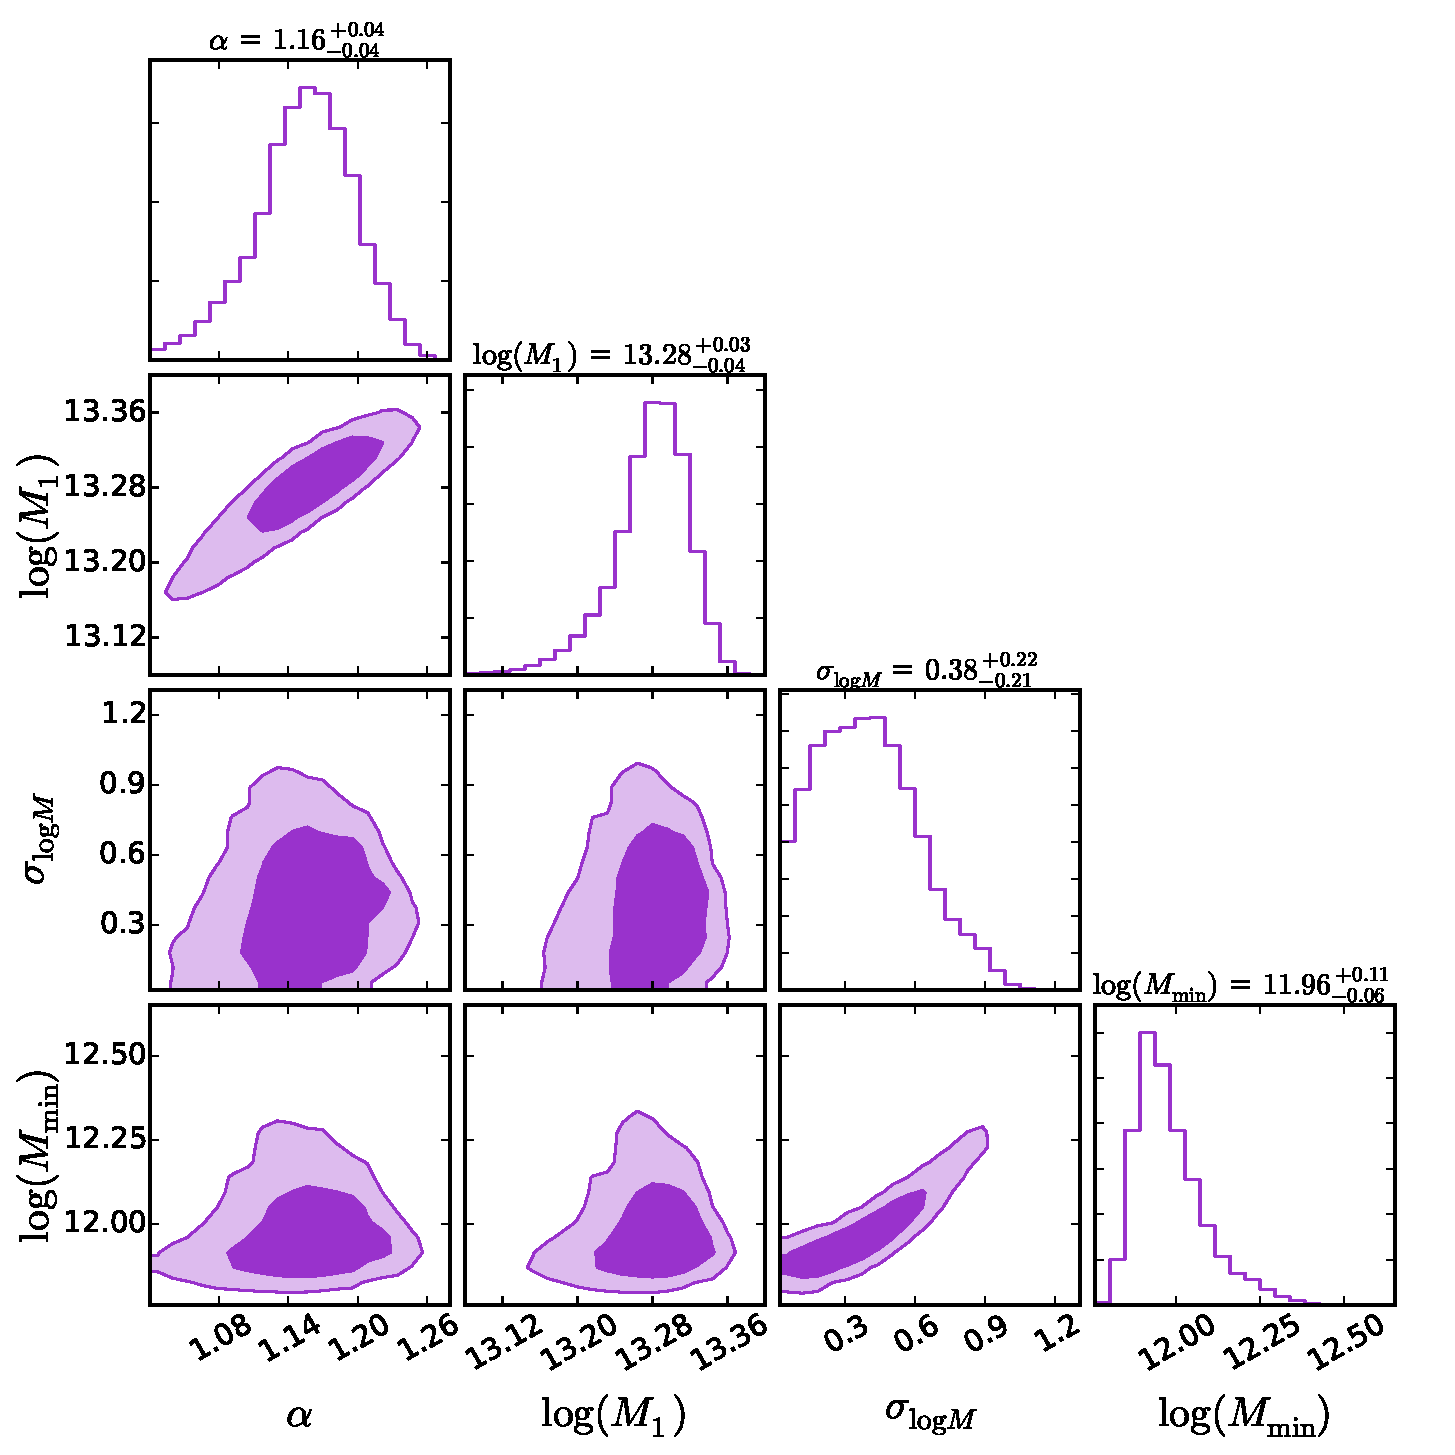
\includegraphics[width=15.0cm]{Mr20_covar_triangle_1.pdf}
\caption{
Two-dimensional marginalized constraints on HOD parameters inferred from 
standard HOD fits to $\wprp(\rp)$ data for the $M_r<-20$ sample. The HOD parameter 
$\log (M_0)$ is extremely poorly constrained by the $\wprp(\rp)$ data and has been 
omitted from this panel. 
}
\label{fig:Mr20triangle}
\end{center}
\end{figure*}


\begin{figure*}
\begin{center}
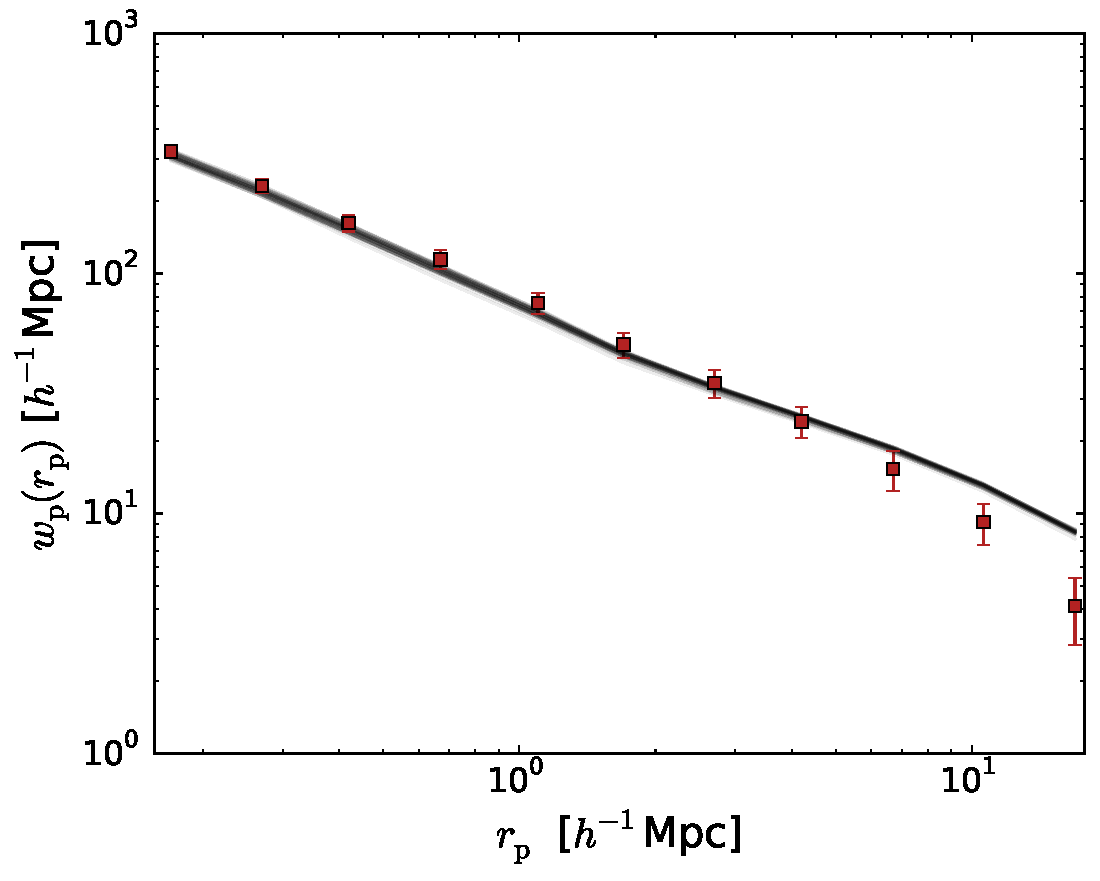
\includegraphics[width=8.3cm]{Mr19samples.pdf}
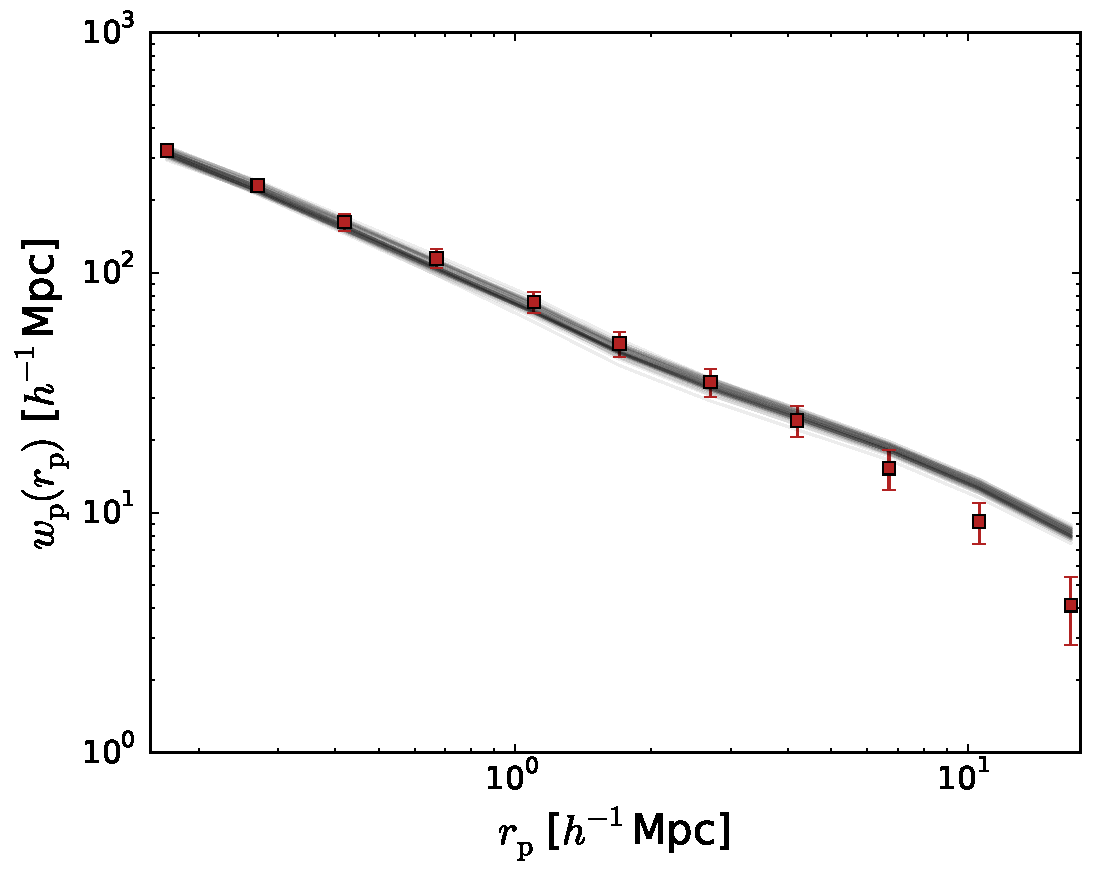
\includegraphics[width=8.3cm]{Mr19ABsamples.pdf}
\caption{
{\bf Left:} The $M_r<-19$ threshold sample projected correlation function with diagonal elements of 
covariance (points with errorbars). The grey lines are 25 randomly-selected HOD models that yield 
$\Delta \chi^2 <1$ compared to the best-fitting model. {\bf Right:} Same as the left panel for decorated 
HOD models that contain parameters to describe the strength of assembly bias.
}
\label{fig:Mr19samples}
\end{center}
\end{figure*}


\begin{figure*}
\begin{center}
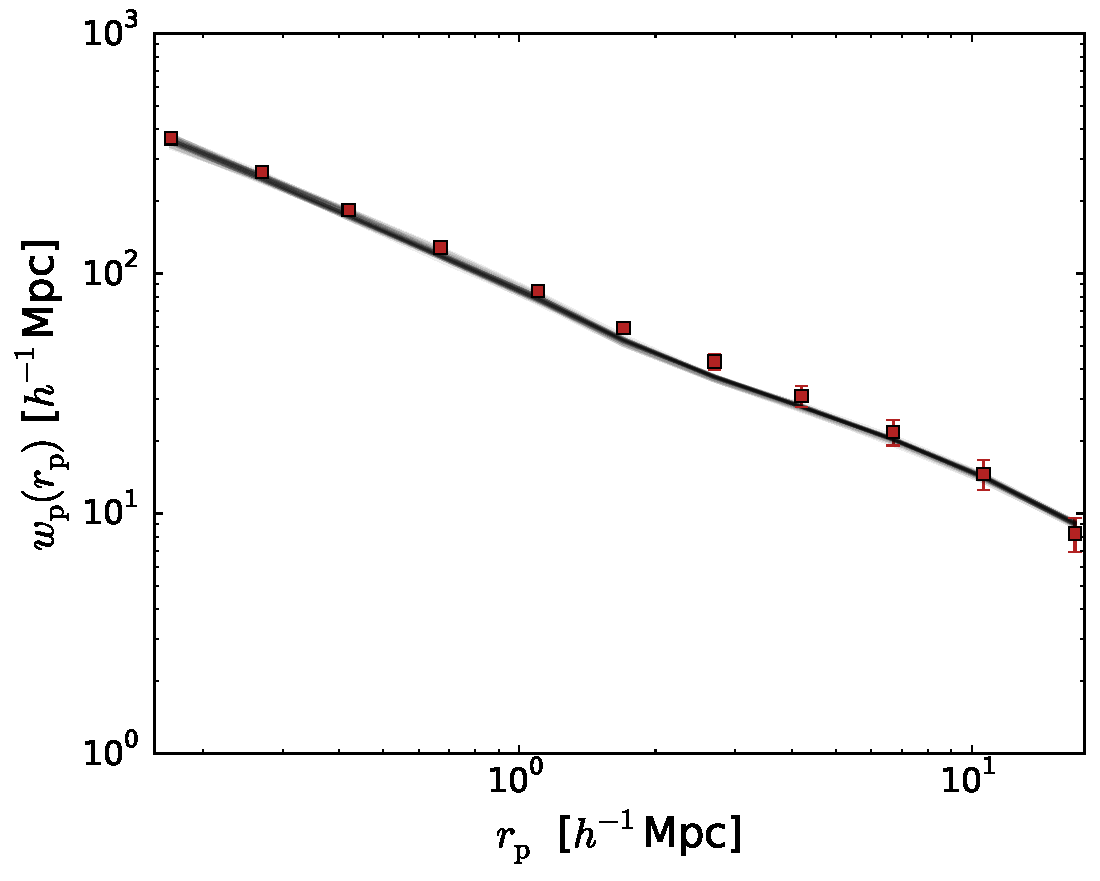
\includegraphics[width=8.3cm]{Mr20samples.pdf}
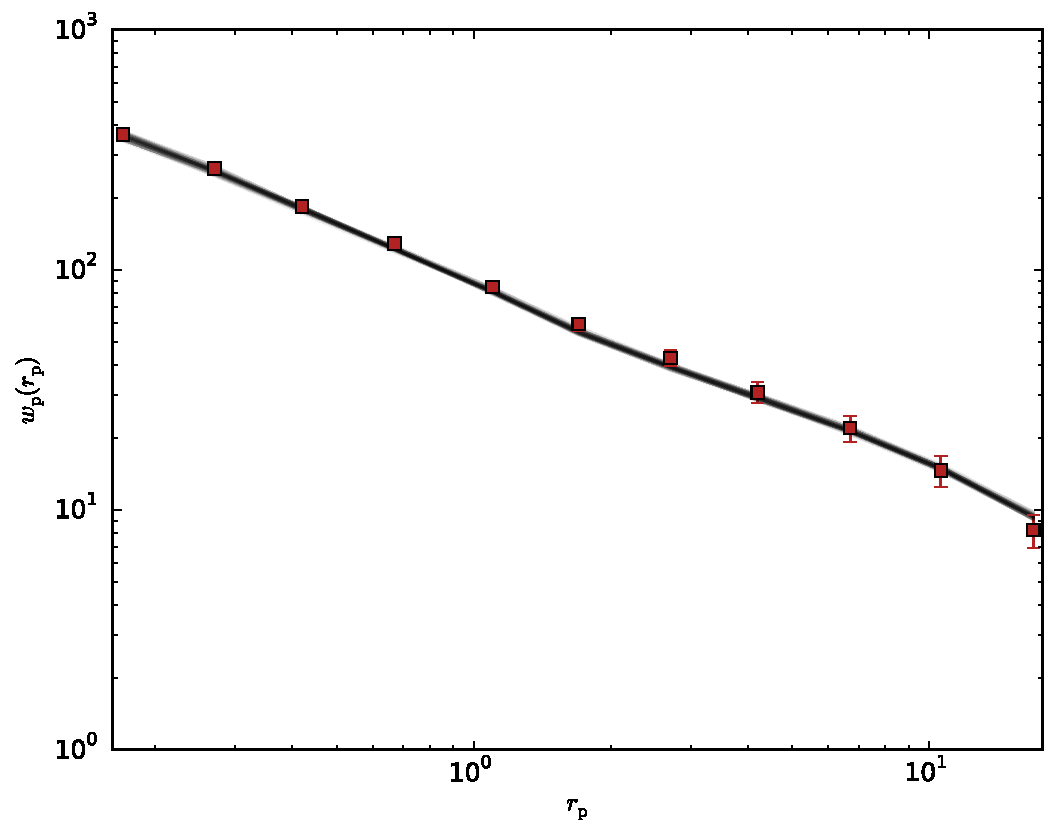
\includegraphics[width=8.3cm]{Mr20ABsamples.pdf}
\caption{
The same as Figure~\ref{fig:Mr19samples}, but for the $M_r<-20$ threshold sample.
}
\label{fig:Mr20samples}
\end{center}
\end{figure*}


\begin{figure*}
\begin{center}
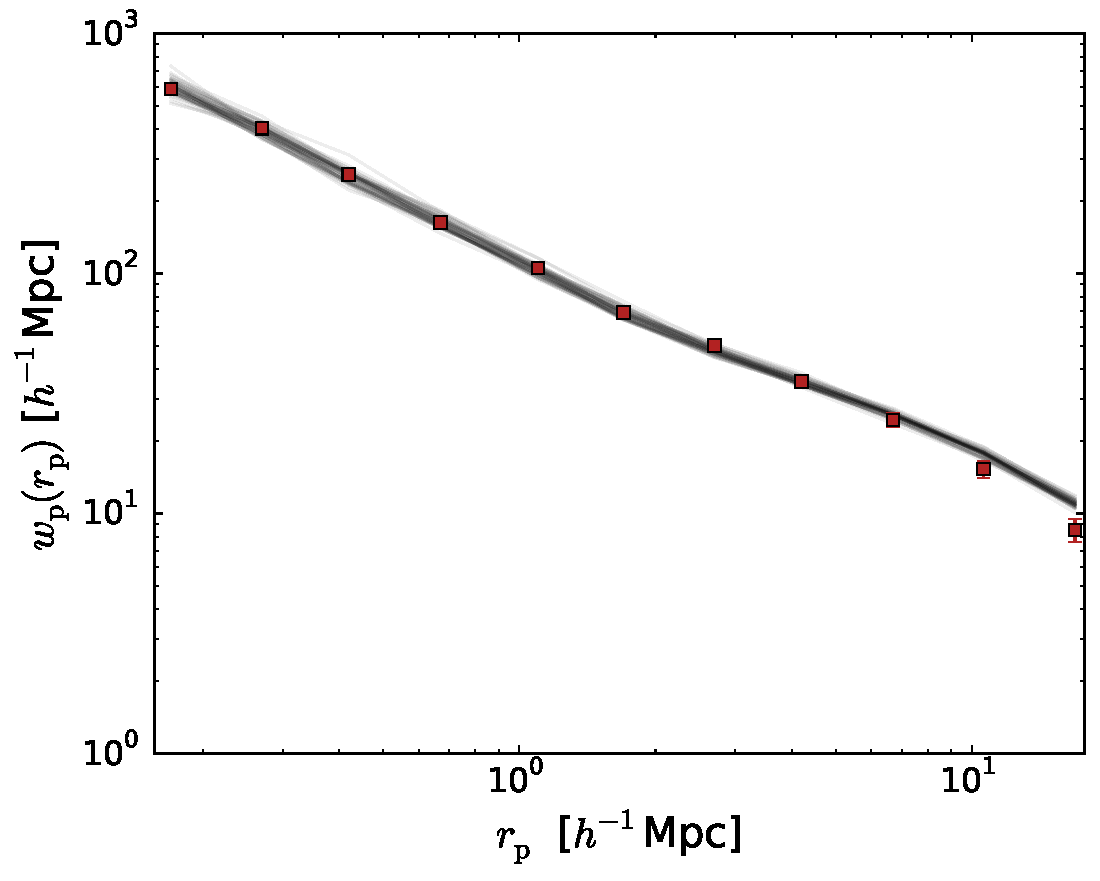
\includegraphics[width=8.3cm]{Mr21samples.pdf}
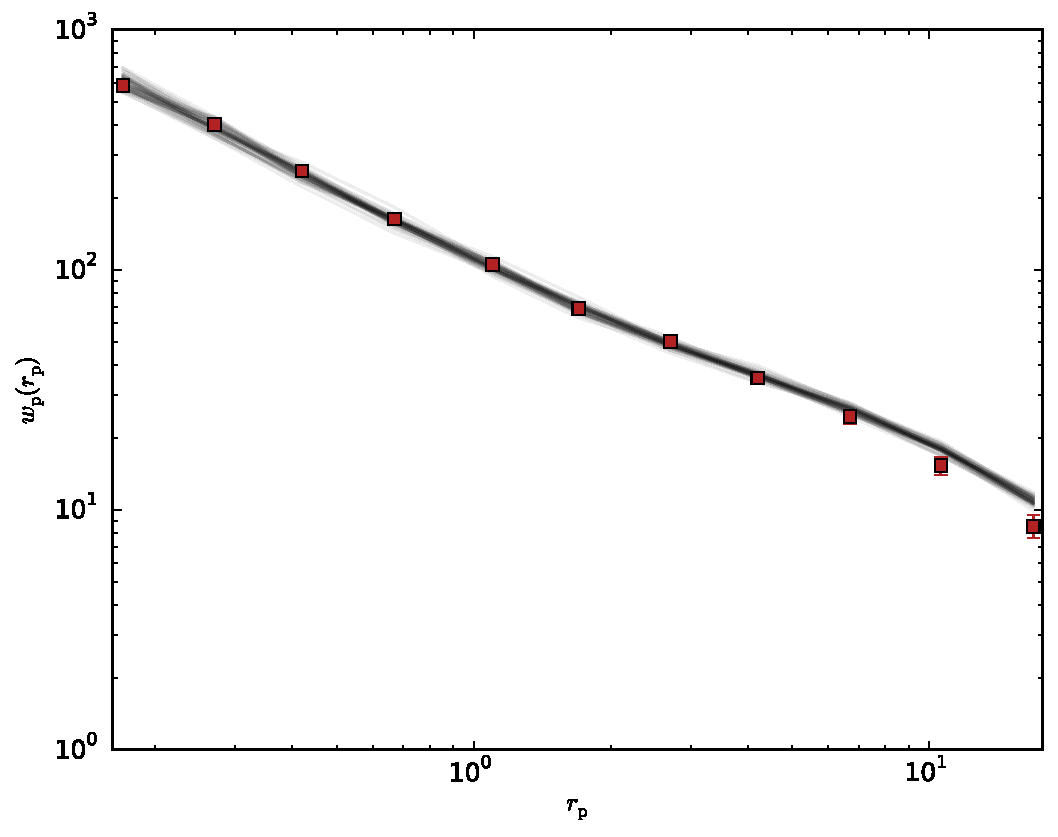
\includegraphics[width=8.3cm]{Mr21ABsamples.pdf}
\caption{
The same as Figure~\ref{fig:Mr19samples}, but for the $M_r<-21$ threshold sample.
}
\label{fig:Mr20samples}
\end{center}
\end{figure*}


%-------------------------
\subsection{Analysis with Decorated HOD}
\label{subsection:ab}
%-------------------------


\begin{figure*}
\begin{center}
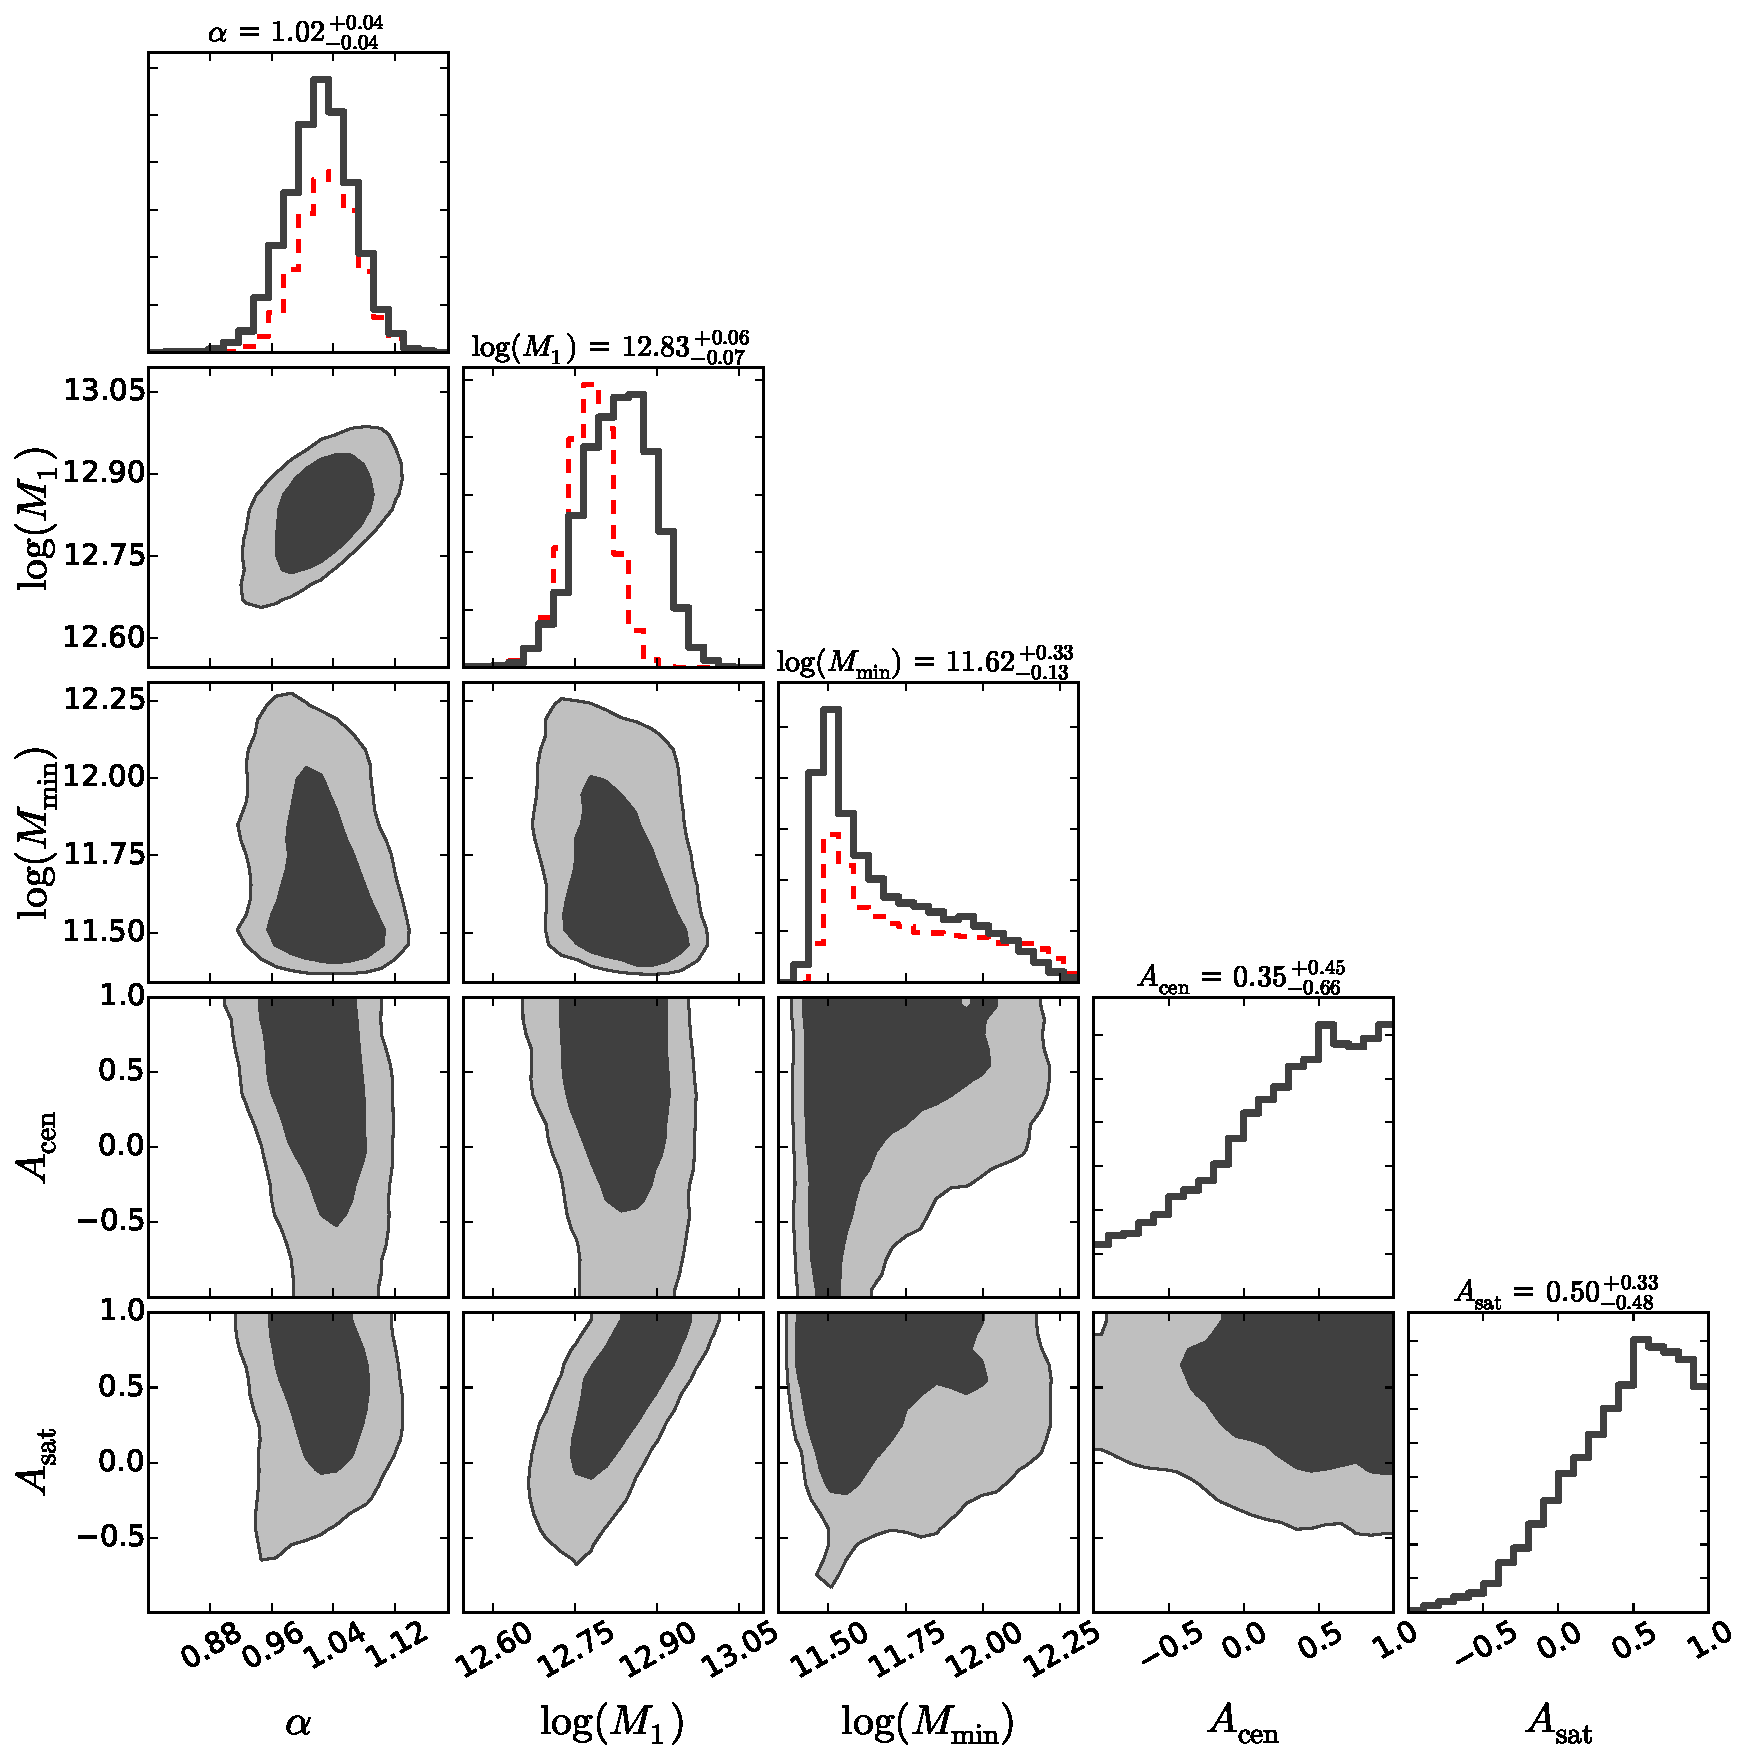
\includegraphics[width=15.0cm]{Mr19ABTri.pdf}
\caption{
Two-dimensional marginalized constraints on decorated HOD parameters inferred from fits 
to $\wprp(\rp)$ data for the $M_r<-19$ sample. The decorated HOD models include a 
two-parameter model for assembly bias. The HOD parameter $\log (M_0)$ is extremely 
poorly constrained by the data and has been suppressed for clarity. Likewise, as in 
Fig.~\ref{fig:Mr20triangle}, $\sigma_{\log M}$ and $\log (M_{\rm min})$ share a 
narrow degeneracy, so we have suppressed $\sigma_{\log M}$ in order to make 
constraints on other parameters more easily visible.
}
\label{fig:Mr19ABtriangle}
\end{center}
\end{figure*}




\begin{figure*}
\begin{center}
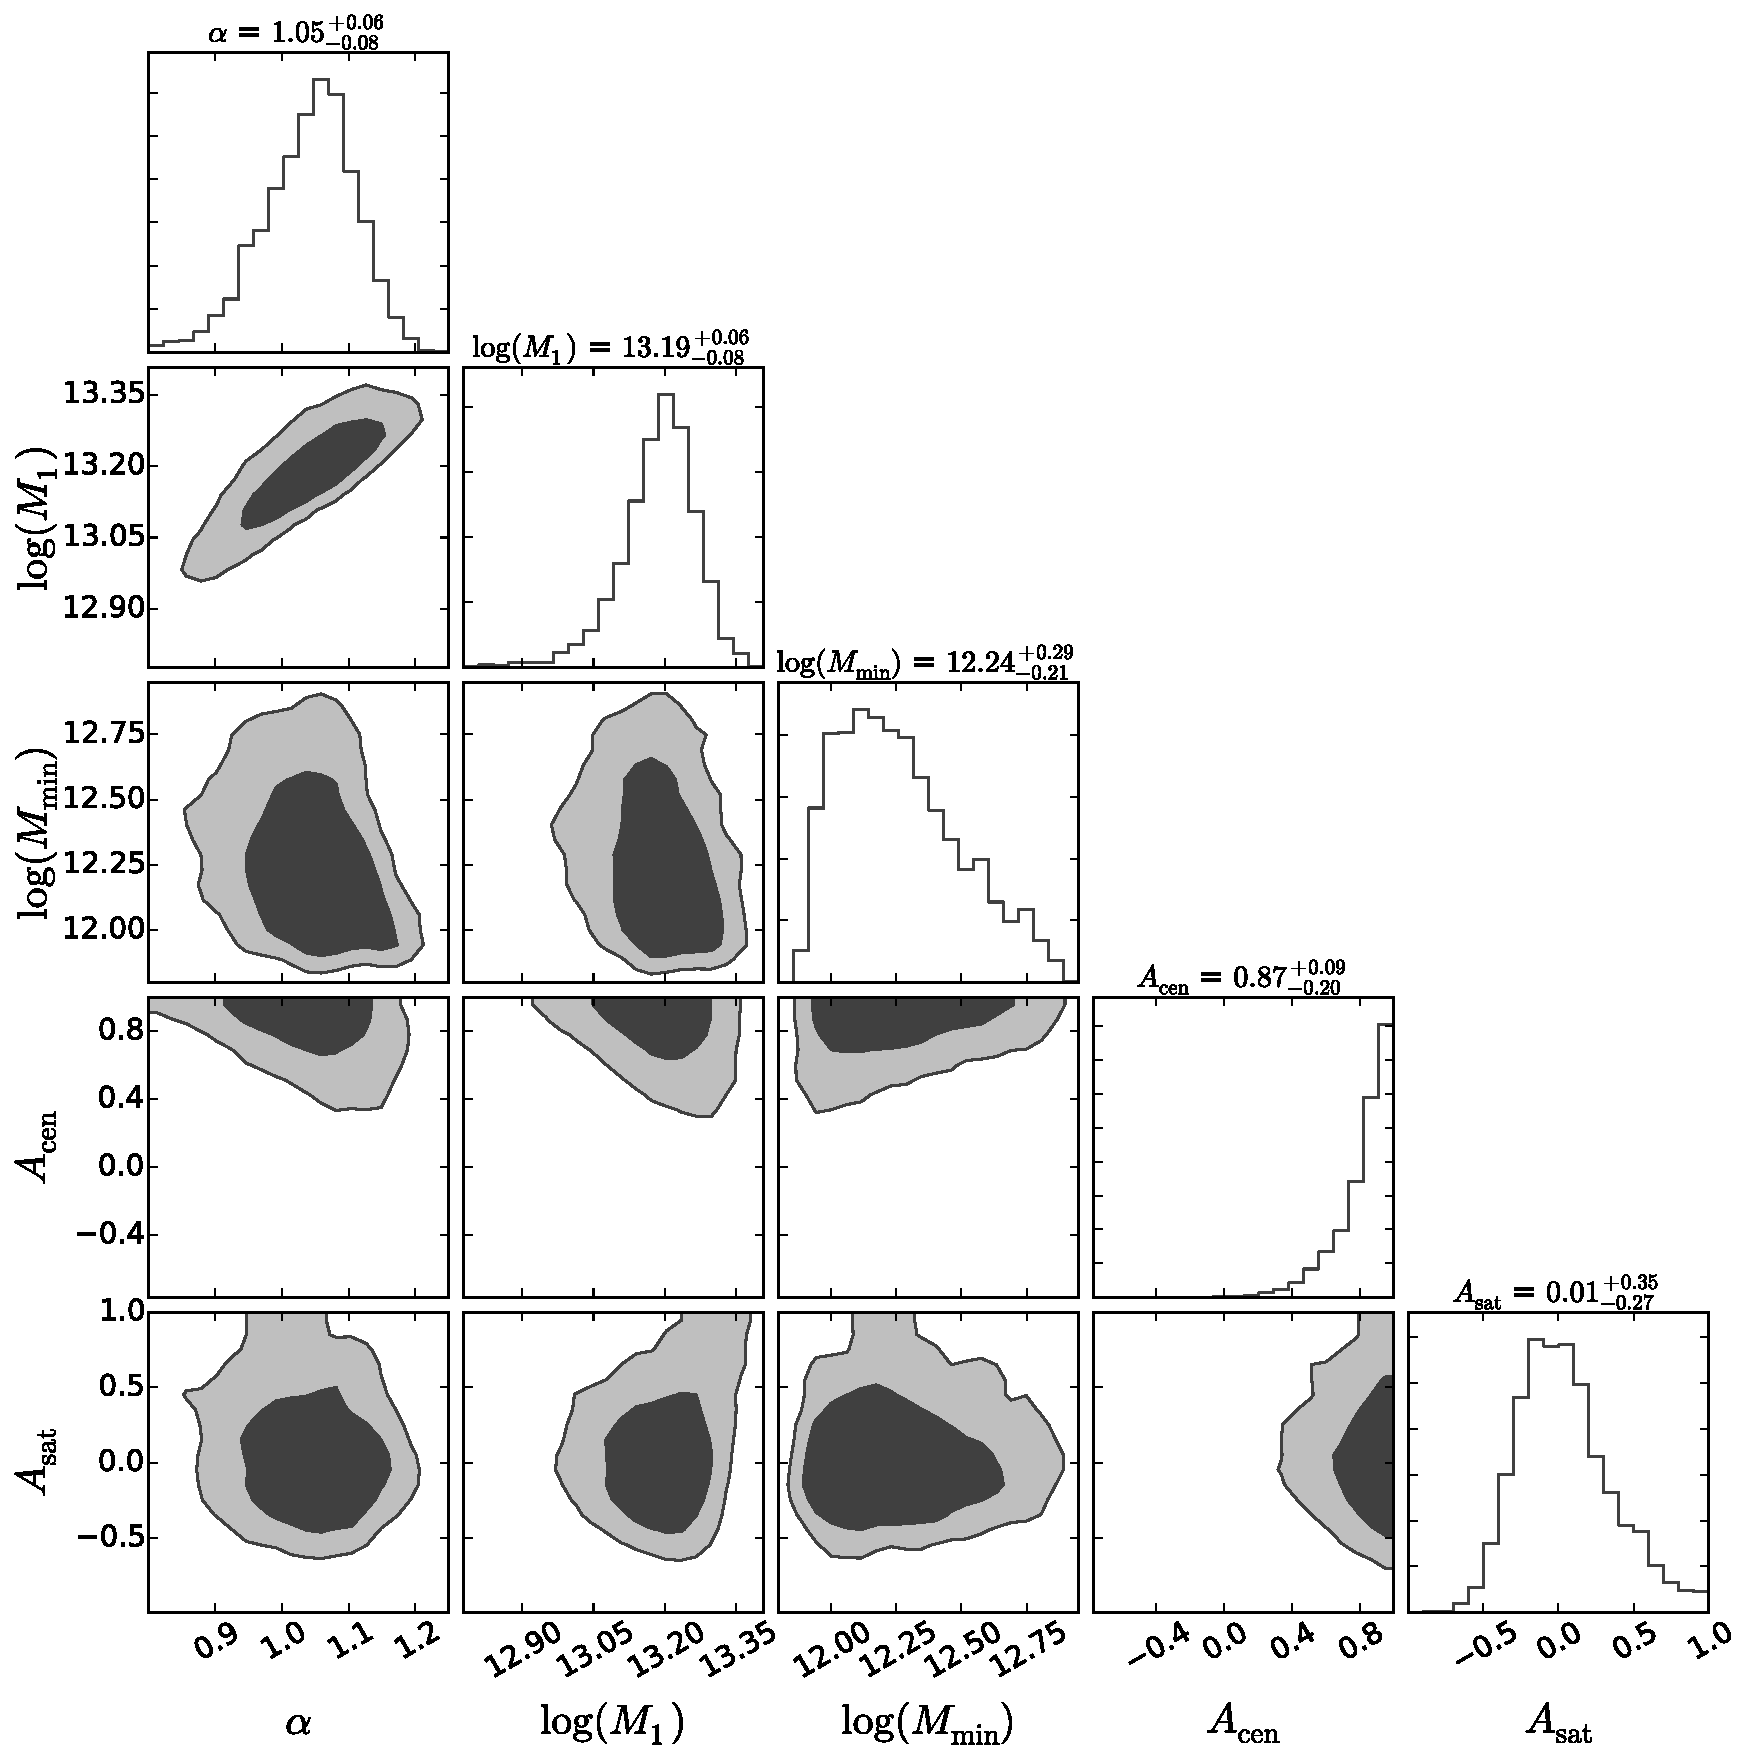
\includegraphics[width=15.0cm]{Mr20ABTri.pdf}
\caption{
The same as Figure~\ref{fig:Mr19ABtriangle}, but for the $M_r<-20$ sample.
}
\label{fig:Mr20ABtriangle}
\end{center}
\end{figure*}



\begin{figure*}
\begin{center}
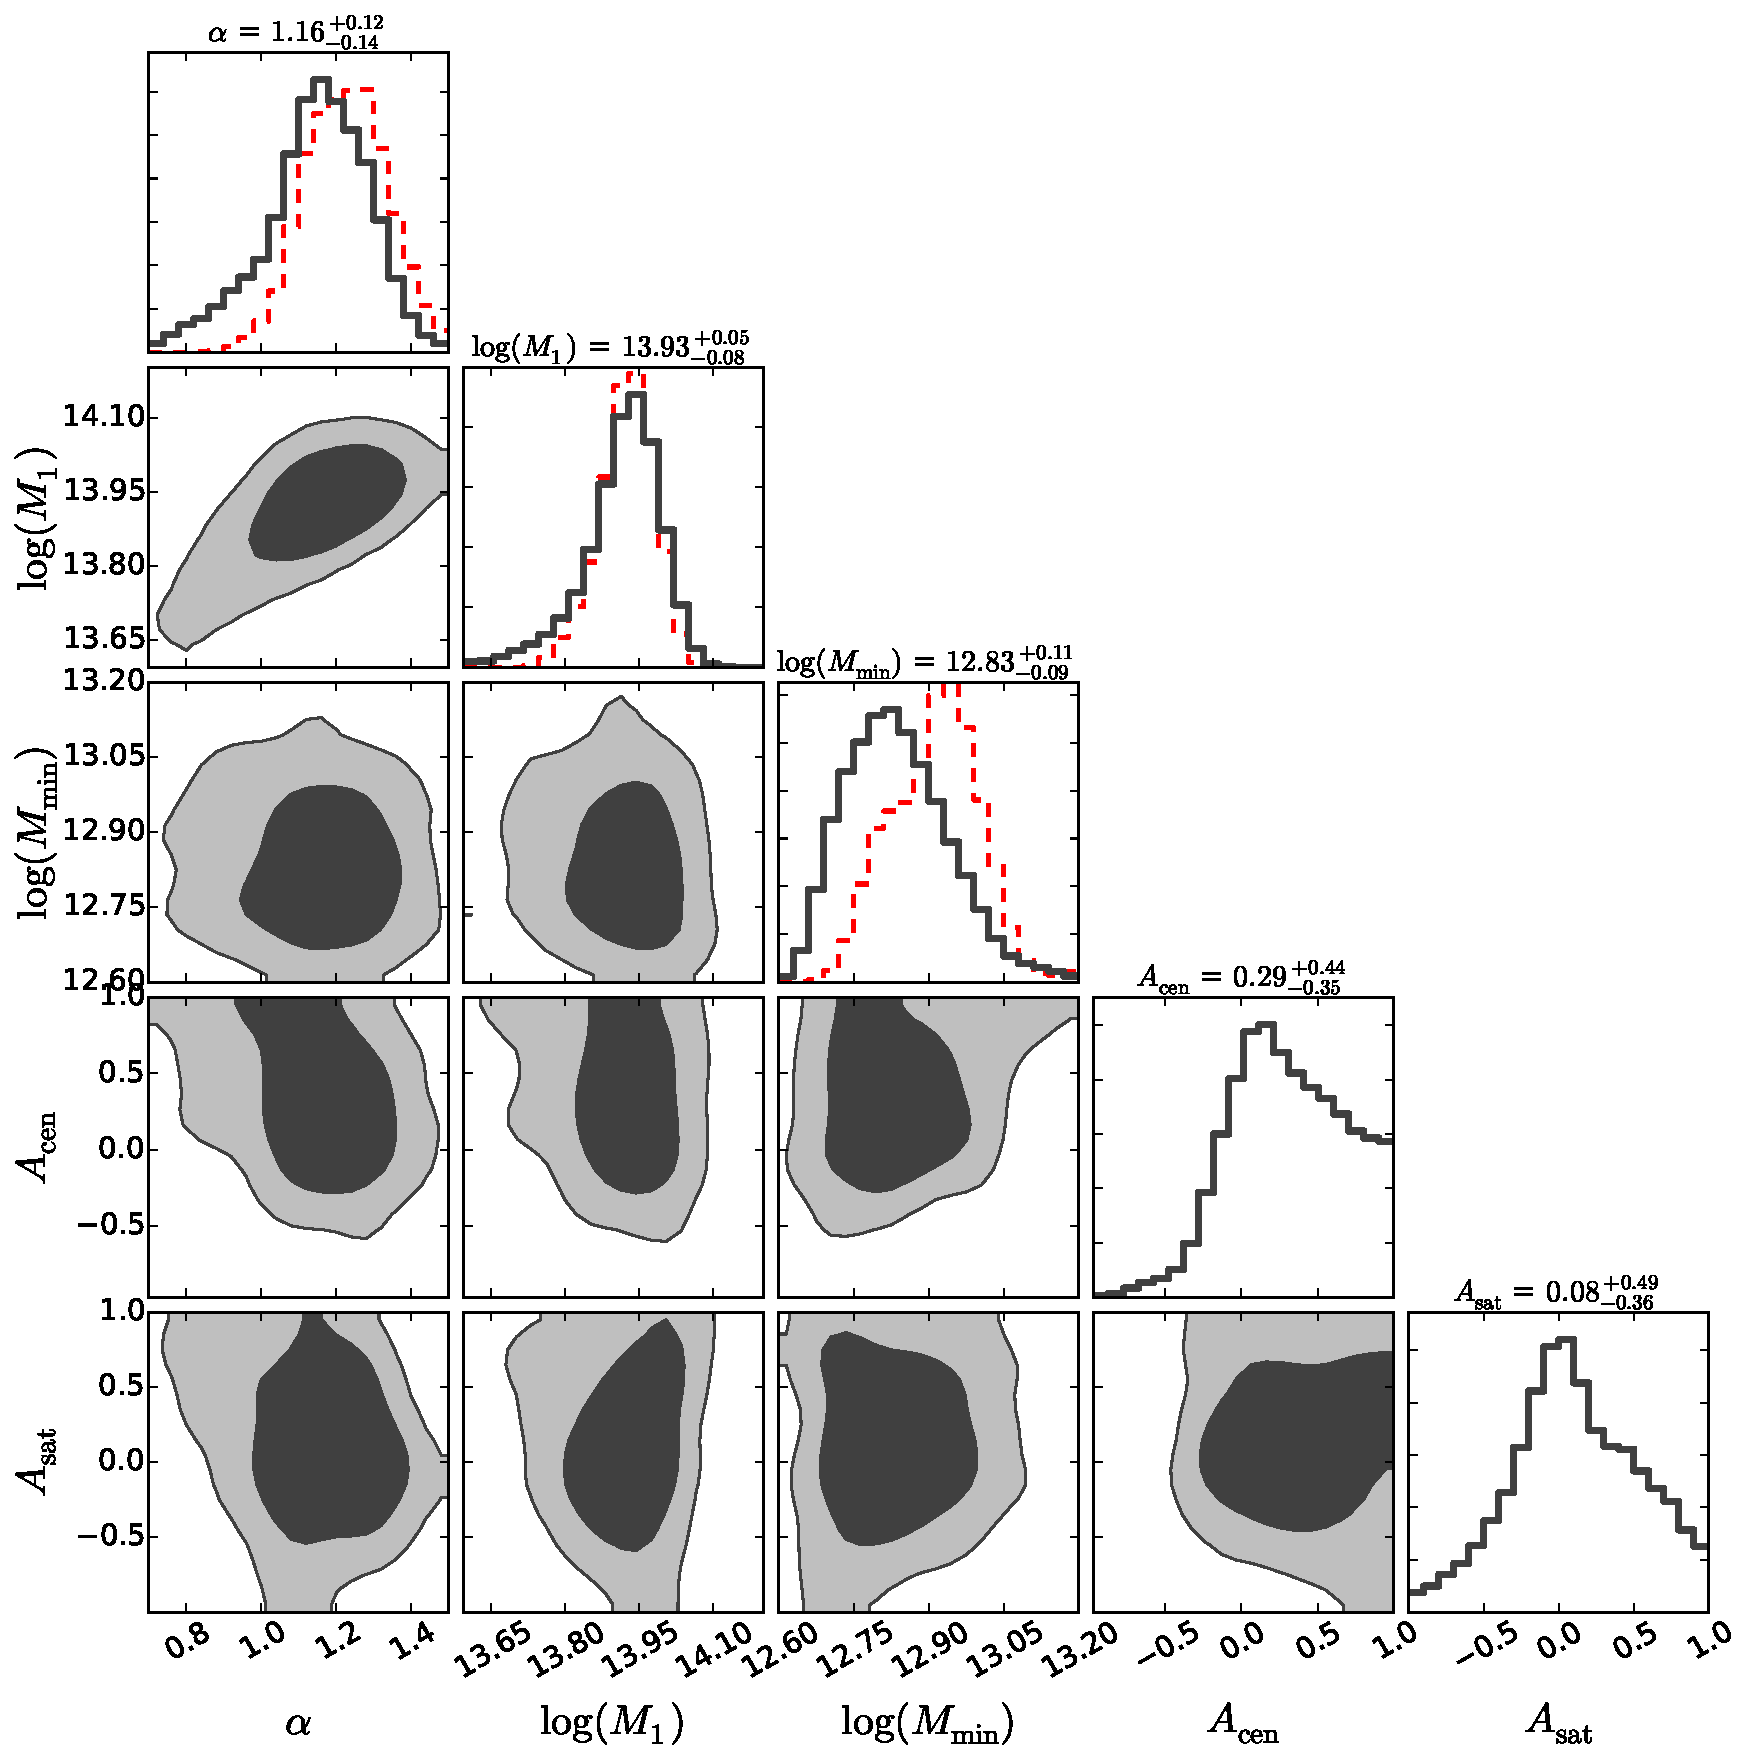
\includegraphics[width=15.0cm]{Mr21ABTri.pdf}
\caption{
The same as Figure~\ref{fig:Mr19ABtriangle}, but for the $M_r<-21$ sample.
}
\label{fig:Mr21ABtriangle}
\end{center}
\end{figure*}



%------------------------------------------------

\bibliography{ms.bib}

%------------------------------------------------
\end{document}
%------------------------------------------------
